%-- coding:UTF-8 --
\documentclass[12pt]{ctexart}

\usepackage{CJK}
\usepackage{booktabs}
\usepackage{graphicx}
\usepackage{multirow}
\usepackage{subfigure}

\begin{document}
% \title{\zihao{1} \bfseries 金属材料热处理实验报告\\
% \begin{large}
% 20CrMn,42CrMo,T10钢不同淬火条件下的微观组织观察和维氏硬度测定
% \end{large}}
\author{陈俊铭、段云智、何阳阳、黄梓煊、卢延昭、陆子良、宣筠铮\\(以姓名拼音排序)}
% \date{\today}


% \maketitle
\newpage
\thispagestyle{empty}
\tableofcontents
\newpage
\setcounter{page}{1}

\section{实验目的}
\begin{itemize}
\item 掌握碳钢的淬火工艺及其应用。
\item 研究冷却条件与钢性能的关系。
\item 观察钢经热处理后的组织,熟悉碳钢经不同热处理后的显微组织及形态特征。
\end{itemize}

\section{实验原理}
\subsection{热处理原理概述}
热处理是一种很重要的金属热加工工艺方法,也是充分发挥金属材料性能潜力的重要手段,它的主要目的是改变钢的性能。所谓热处理是将钢在固态下通过加热、保温与冷却的方法改变其组织与性能的工艺。主要包括退火、正火、淬火及回火。本实验主要涉及正火与淬火工艺。
\subsubsection{正火}
正火工艺 将钢加热到${A_{{c_3}}}$或 ${A_{{c_m}}}$以上30-50℃ ,保温一定时间,然后在空气中冷却的工艺方法,称为正火。正火的速度比退火快,可获得较为细密的索氏体组织,因而比退火组织具有较高的强度和硬度。
\subsubsection{淬火}
\paragraph{}
 钢的淬火是将钢加热到相变温度(${A_{{c_3}}}$或${A_{{c_1}}}$) 以上,保温一定时间后,以快速冷却的一种工艺,通常淬火钢的基体是马氏体。将钢加热到${A_{{c_3}}}$ 以上称为完全淬火 , 加热到${A_{{c_1}}}$ 以 上为不完全退火。
\paragraph{}
 淬火冷却方法非常重要,一方面冷却速度要大于临界冷却速度,以保证全部得到马氏体组织;另一方面冷却应尽量缓慢,以减少内应力,避免变形和开裂。为了解决上述矛盾,可以采用不同的冷却介质和方法,使淬火工件在奥氏体最不稳定的温度范围内(650—550℃)快冷,超过临界冷却速度,而在Ms(300—100℃)点以下温度时冷却较慢,理想的冷却速度如图 \ref{cuihuoquxian} 所示。
\begin{figure}[h]
  \centering
  % Requires \usepackage{graphicx}
  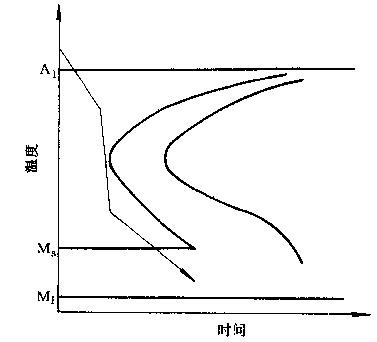
\includegraphics[width=5cm]{cuihuoquxian.jpg}\\
  \caption{淬火时的理想冷却曲线示意图}
  \label{cuihuoquxian}
\end{figure}



\paragraph{}
 冷却介质一般用 油、水和盐水,这三种介质的冷却能力依次增强。由于碳钢的含碳量不同、淬火加热温度不 同、 冷却介质不同时所得到的组织不同,因而性能也不同。本实验采用的冷却剂为水与矿物油。
\begin{table}[ht!]
  \centering
  \begin{tabular}{|c|c|c|}
     \hline
     % after \\: \hline or \cline{col1-col2} \cline{col3-col4} ...
     \multirow{2}{*}{冷却介质}& \multicolumn{2}{c|}{冷却速度℃/s} \\
     \cline{2-3}
     &650—550℃区间& 300—200℃区间 \\
     \hline
     水(26℃)& 500 & 270 \\
     \hline
     矿物油 & 150 & 30 \\
     \hline
   \end{tabular}
  \caption{水及矿物油的冷却能力}
\end{table}
\subsection{热处理微观组织}
\subsubsection{正火组织}
正火的冷却速度大于退火的冷却速度,因此,在相同含碳量情况下,正火比退火的组织要细,得到的组织为:索氏体+铁素体(呈断续网状分布),见图 \ref{zhenghuo}。
\begin{figure}[ht!]
  \centering
  % Requires \usepackage{graphicx}
  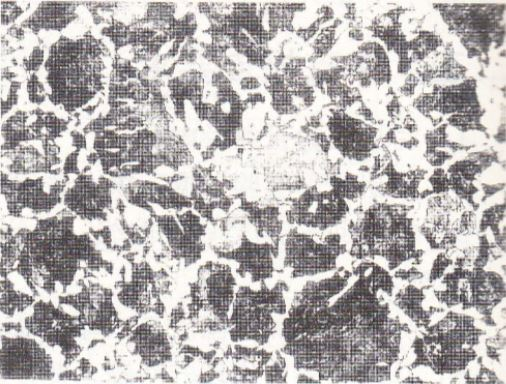
\includegraphics[width=5cm]{zhenghuo.jpg}\\
  \caption{45钢正火组织 400×}\label{zhenghuo}
\end{figure}

\subsubsection{淬火组织}
\paragraph{马氏体组织}
马氏体是奥氏体在冷却速度大于临界冷却速度到${M_{s}}$ 温度得到的转变产物,有两种典型形态:板条马氏体和片状马氏体。
\subparagraph{板条马氏体}
板条马氏体是一种低碳马氏体,其显微组织特征事由一束束相互平行排列的板条状组织成群分布,在一个奥氏体晶粒内可能有几个不同取向的马氏体群,在一个奥氏体晶粒内可能有几个不同取向的马氏体群。图 \ref{ditangangcuihuo}为低碳钢的淬火组织。
\begin{figure}[ht!]
  \centering
  % Requires \usepackage{graphicx}
  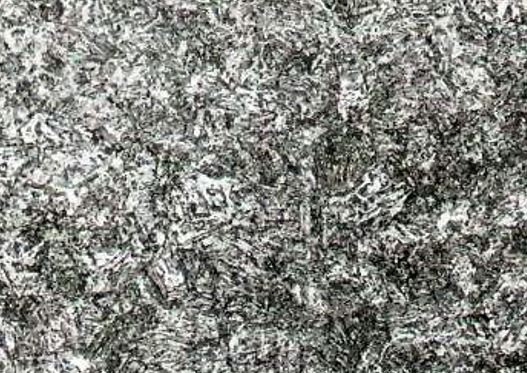
\includegraphics[width=5cm]{bantiaomashiti.jpg}\\
  \caption{低碳钢的淬火组织}\label{ditangangcuihuo}
\end{figure}
\subparagraph{片状马氏体}
片状马氏体是一种高碳马氏体,其显微组织的主要特征是在光学显微镜下呈现针状或竹叶状,高碳钢经过高温淬火得到粗大的针状马氏体,其立体形貌是凸透镜状。图 \ref{gaotangangcuihuo}为高碳钢的淬火组织。
\begin{figure}[ht!]
  \centering
  % Requires \usepackage{graphicx}
  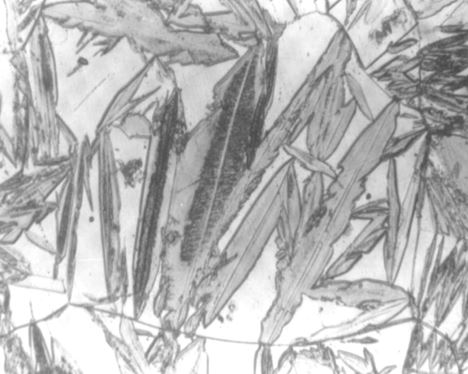
\includegraphics[width=5cm]{pianzhuangmashiti.jpg}\\
  \caption{Fe-32Ni合金的片状马氏体组织}\label{gaotangangcuihuo}
\end{figure}
\paragraph{油冷组织}
由于油冷的冷速较水冷慢,沿奥氏体晶界首先析出屈式体,并呈现网状分布。随后剩余奥氏体转变成为混合马氏体。图 \ref{youlengcuihuo}为45钢的油冷组织。
\begin{figure}[ht!]
  \centering
  % Requires \usepackage{graphicx}
  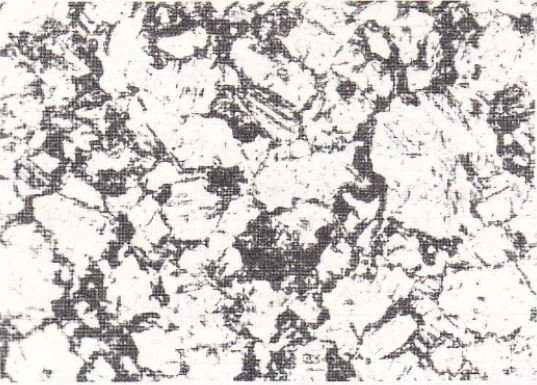
\includegraphics[width=5cm]{youlengcuihuo.jpg}\\
  \caption{45钢油 冷 组 织 500×}\label{youlengcuihuo}
\end{figure}

\section{实验材料和仪器}
\subsection{实验材料}
实验采用材料为高约15mm,直径$\phi$约20mm的圆柱形20CrMn,42CrMo,T10钢样品,其化学成分见表 \ref{huaxuechengfen}。

\begin{table}[ht!]
  \centering
  \caption{20CrMn,42CrMo,T10钢的化学成分}
  \label{huaxuechengfen}
  \begin{tabular}{cccccc}
    \toprule
    &C(\%)&Si(\%)&Mn(\%)&Cr(\%)&Mo(\%)\\
    \midrule
    20CrMo&0.17-0.24&0.17-0.37&0.40-0.70&0.80-1.10&0.15-0.25\\
    42CrMo&0.38-0.45&0.17-0.37&0.50-0.80&0.90-1.20&0.15-0.2\\
    T10   &0.95-1.04&≤0.35    &≤0.40    &≤0.25    &≤0.20\\
    \bottomrule
  \end{tabular}
\end{table}

\subsection{实验仪器}
\begin{itemize}
  \item 箱式电阻炉
  \item 维氏硬度计
  \item 金相显微镜及电子扫描显微镜
  \item 抛光膏及抛光机
  \item 浸蚀剂、酒精、玻璃器皿、竹夹子、脱脂棉、滤纸等
\end{itemize}

\section{实验步骤}
\subsection{淬火}
\subsubsection{加热温度}
根据表 \ref{huaxuechengfen}提供的化学成分和图 \ref{cuihuowendu}综合考量,设定加热温度为850℃.
\newpage
\begin{figure}[h]
  \centering
  % Requires \usepackage{graphicx}
  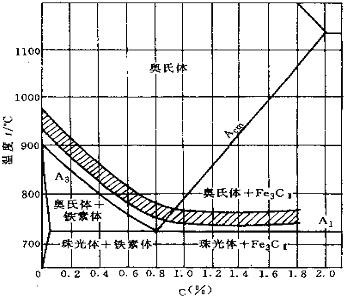
\includegraphics[width=7cm]{cuihuowendu.jpg}\\
  \caption{淬火的加热温度范围}\label{cuihuowendu}
\end{figure}

\subsubsection{加热时间}
淬火加热保温时间按下列经验公式估算:

\[t = \alpha  \cdot K \cdot H\]

\paragraph{}
式中t—保温时间(min);

    $\alpha$—加热系数(min/mm) (对于800℃-900℃箱式炉加热一般可以取1.0-1.2);

    $K$—工件装炉方式修正系数(一般 $K$ = 1~1.5);

    $H$—工件有效厚度(mm)(尺寸最小部位)。
\paragraph{}
结合样品尺寸计算可得样品至少需要加热15min。
\subsubsection{具体操作}
把样品放入箱式电阻内恒温区的耐火砖上,调节加热温度,待测温仪显示为850℃时开始计时,保温15min后,用火钳夹出样品迅速放入水、油槽中并剧烈搅拌,使样品能淬透。正火样品放置在防火砖上待其空冷结束。
\subsection{显微组织观察}
\paragraph{}
用一套金相砂纸在玻璃板上先粗后细逐号磨光。注意每换上一号细一些的砂纸时,将磨光方向转换90°,以便于观察原磨痕的消除情况。最后,金相样品抛光机上细抛,使样品表面达到光亮如镜的光洁度。注意手持样品应用力均匀,用力也不宜过大。
\paragraph{}
将抛光好的样品,直接在显微镜下观察,应基本上没有磨痕和磨坑,而无法观察到晶界、各类相和组织。本实验采用化学浸蚀法,将浸蚀液(4\%硝酸酒精)和纯酒精各倒入一个玻璃器皿中,用竹夹子夹脱脂棉、蘸浸蚀液在样品表面擦试,当光亮镜面呈浅灰白色,立即用水冲洗,并用酒精擦洗后经吸水纸吸干。
\paragraph{}
制备好的样品分别用光学显微镜在100和500倍不同放大倍数下,用扫描电子显微镜在1000和2000倍下观察组织,并拍摄图片。
\subsection{测定维氏硬度}
\paragraph{}
然后,将样品放在维式硬度计的载物台上,调整焦距,在试样上不同位置取三个点个点,三个点计入数据,若三个点硬度值相差不大说明组织较为均匀,最后对三个测量值求平均值。

\section{实验结果与分析}
\subsection{显微组织分析}
\subsubsection{20CrMo钢}
20CrMo钢的CCT曲线如图 \ref{cct20}所示,并根据水冷、油冷及空冷的冷却速度,在图 \ref{cct20}中大致画出冷却曲线:
\begin{figure}[h]
  \centering
  % Requires \usepackage{graphicx}
  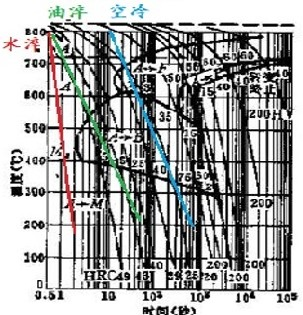
\includegraphics[width=7cm,height=7cm]{cct20.jpg}\\
  \caption{20CrMo钢的CCT曲线}\label{cct20}
\end{figure}
\paragraph{水冷}
水淬的冷却速度约为500℃/s,由CCT曲线可知,其冷却速度大于临界淬火速度,可使奥氏体不发生珠光体相变而获得完全马氏体(包括残余奥氏体)。

\begin{figure}[h]
  \centering
  \subfigure[光学显微镜500×]{
    \label{20shuiguang}
    \begin{minipage}{6cm}
    \centering
    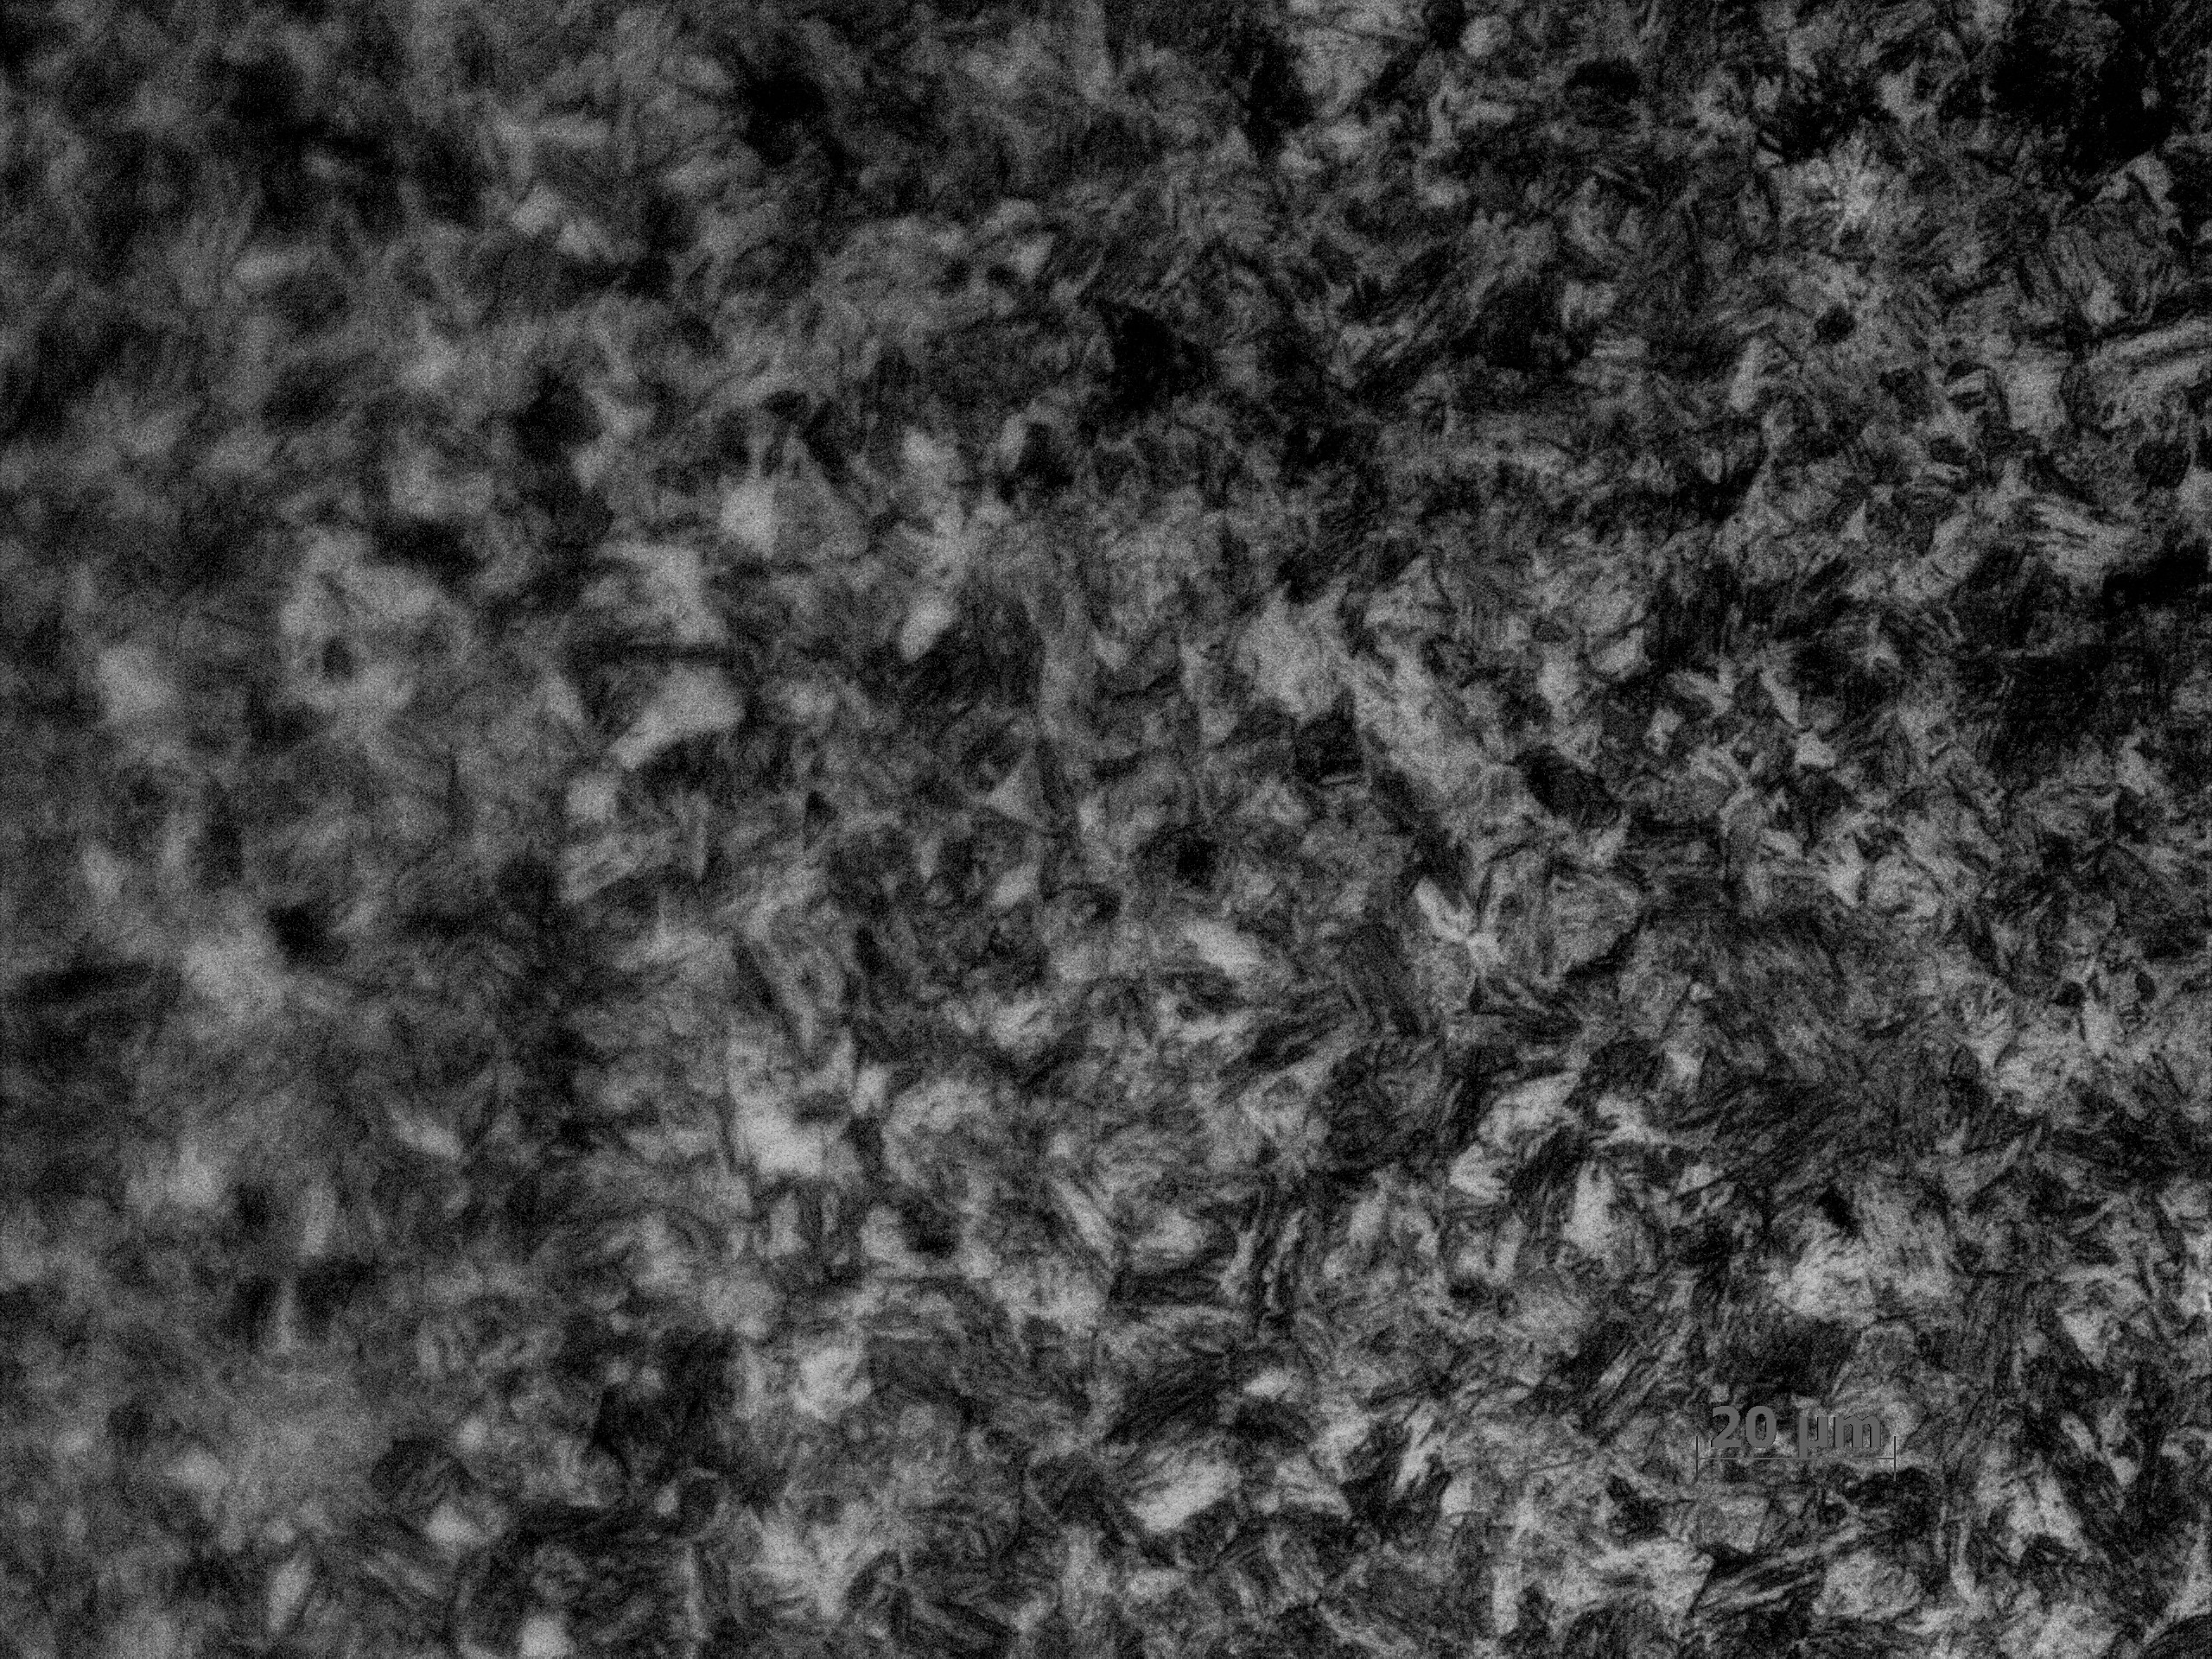
\includegraphics[width=6cm]{20waterguang.jpg}
    \end{minipage}
  }
  \subfigure[扫描电子显微镜5000×]{
    \label{20shuidian}
    \begin{minipage}{6cm}
    \centering
    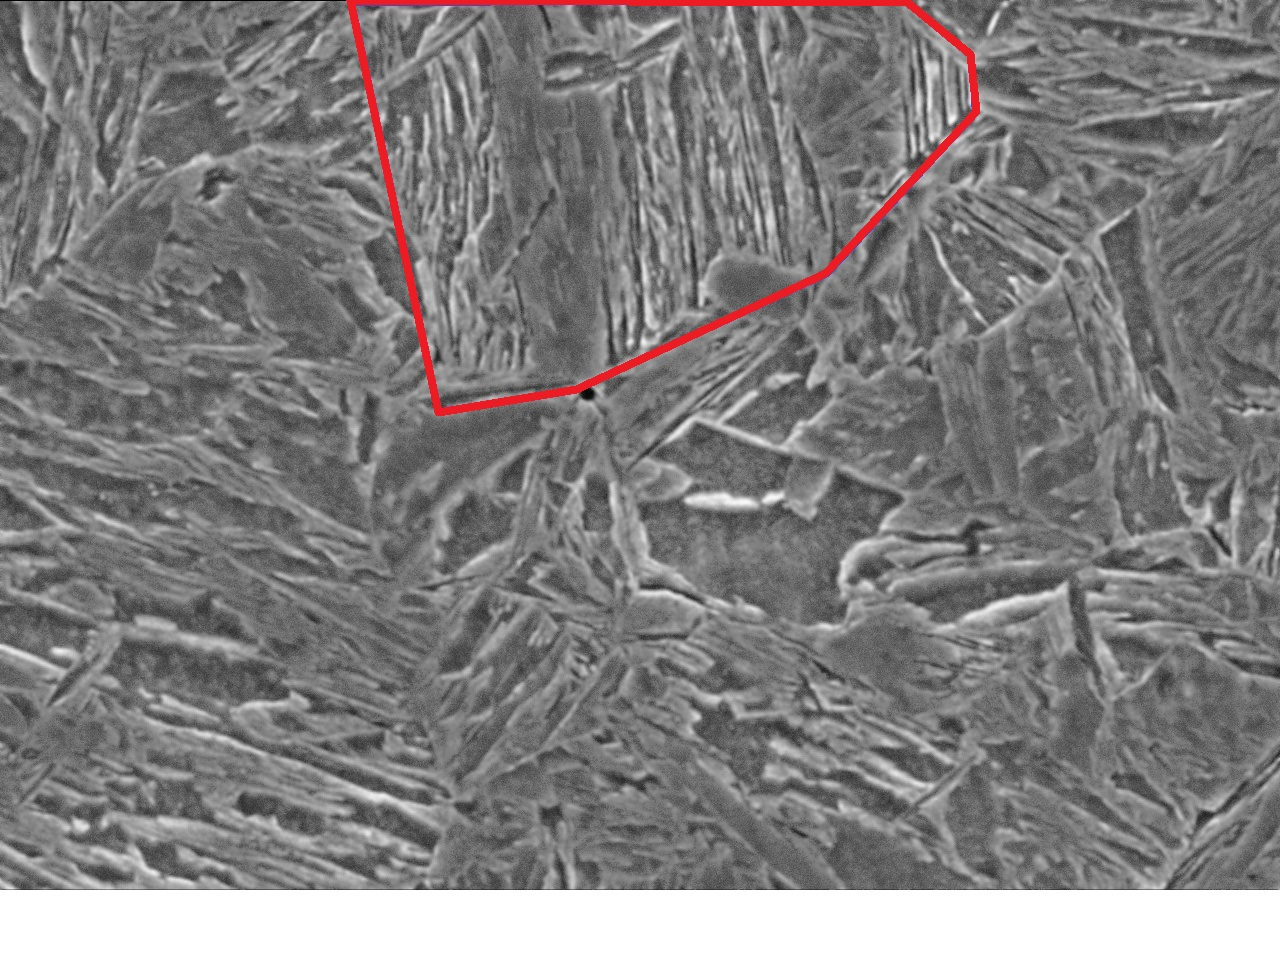
\includegraphics[width=6cm]{20waterdian.jpg}
    \end{minipage}
  }
  \caption{20CrMo钢水冷金相照片}
  \label{20water}
\end{figure}
\subparagraph{板条状马氏体}
板条状马氏体是低碳钢中形成的一种典型的马氏体组织,因其显微组织是由许多成群的板条组成,故称为板条状马氏体。因为这种马氏体的亚结构主要为位错,通常也称为位错型马氏体。其马氏体晶粒呈一定角度相交,在图 \ref{20water}中可以较清晰的看出。
\subparagraph{同位向束\  板条}
板条状马氏体由板条群所组成,一个原始奥氏体晶粒内可有几个板条群。板条群由若干尺寸大致相同的板条在空间位向大致平行排列所组成,一个板条群又可分成几个平行的区域,称为同位向束。每个同位向束由若干个平行板条所组成,每个板条为一个马氏体单晶体,金相呈现为黑白交替的块,在图 \ref{20water}电镜照片框中可以很清晰清晰的看出平行板条和其黑白交替,马氏体板条多被连续的残余奥氏体薄膜所隔开。
\subparagraph{表面浮突}
由于马氏体形成是以切变方式进行的,且一边相对凸起,一边相对凹陷,使表面出现浮突现象,且在板条状马氏体中,浮突呈现帐篷型。

\paragraph{油冷}
水淬的冷却速度约为150℃/s,由CCT曲线可知,其冷却速度小于临界淬火速度,可使奥氏体不发生珠光体相变而获得完全马氏体(包括残余奥氏体)。
\newpage
\begin{figure}[h]
  \centering
  \subfigure[光学显微镜500×]{
    \label{20youguang}
    \begin{minipage}{6cm}
    \centering
    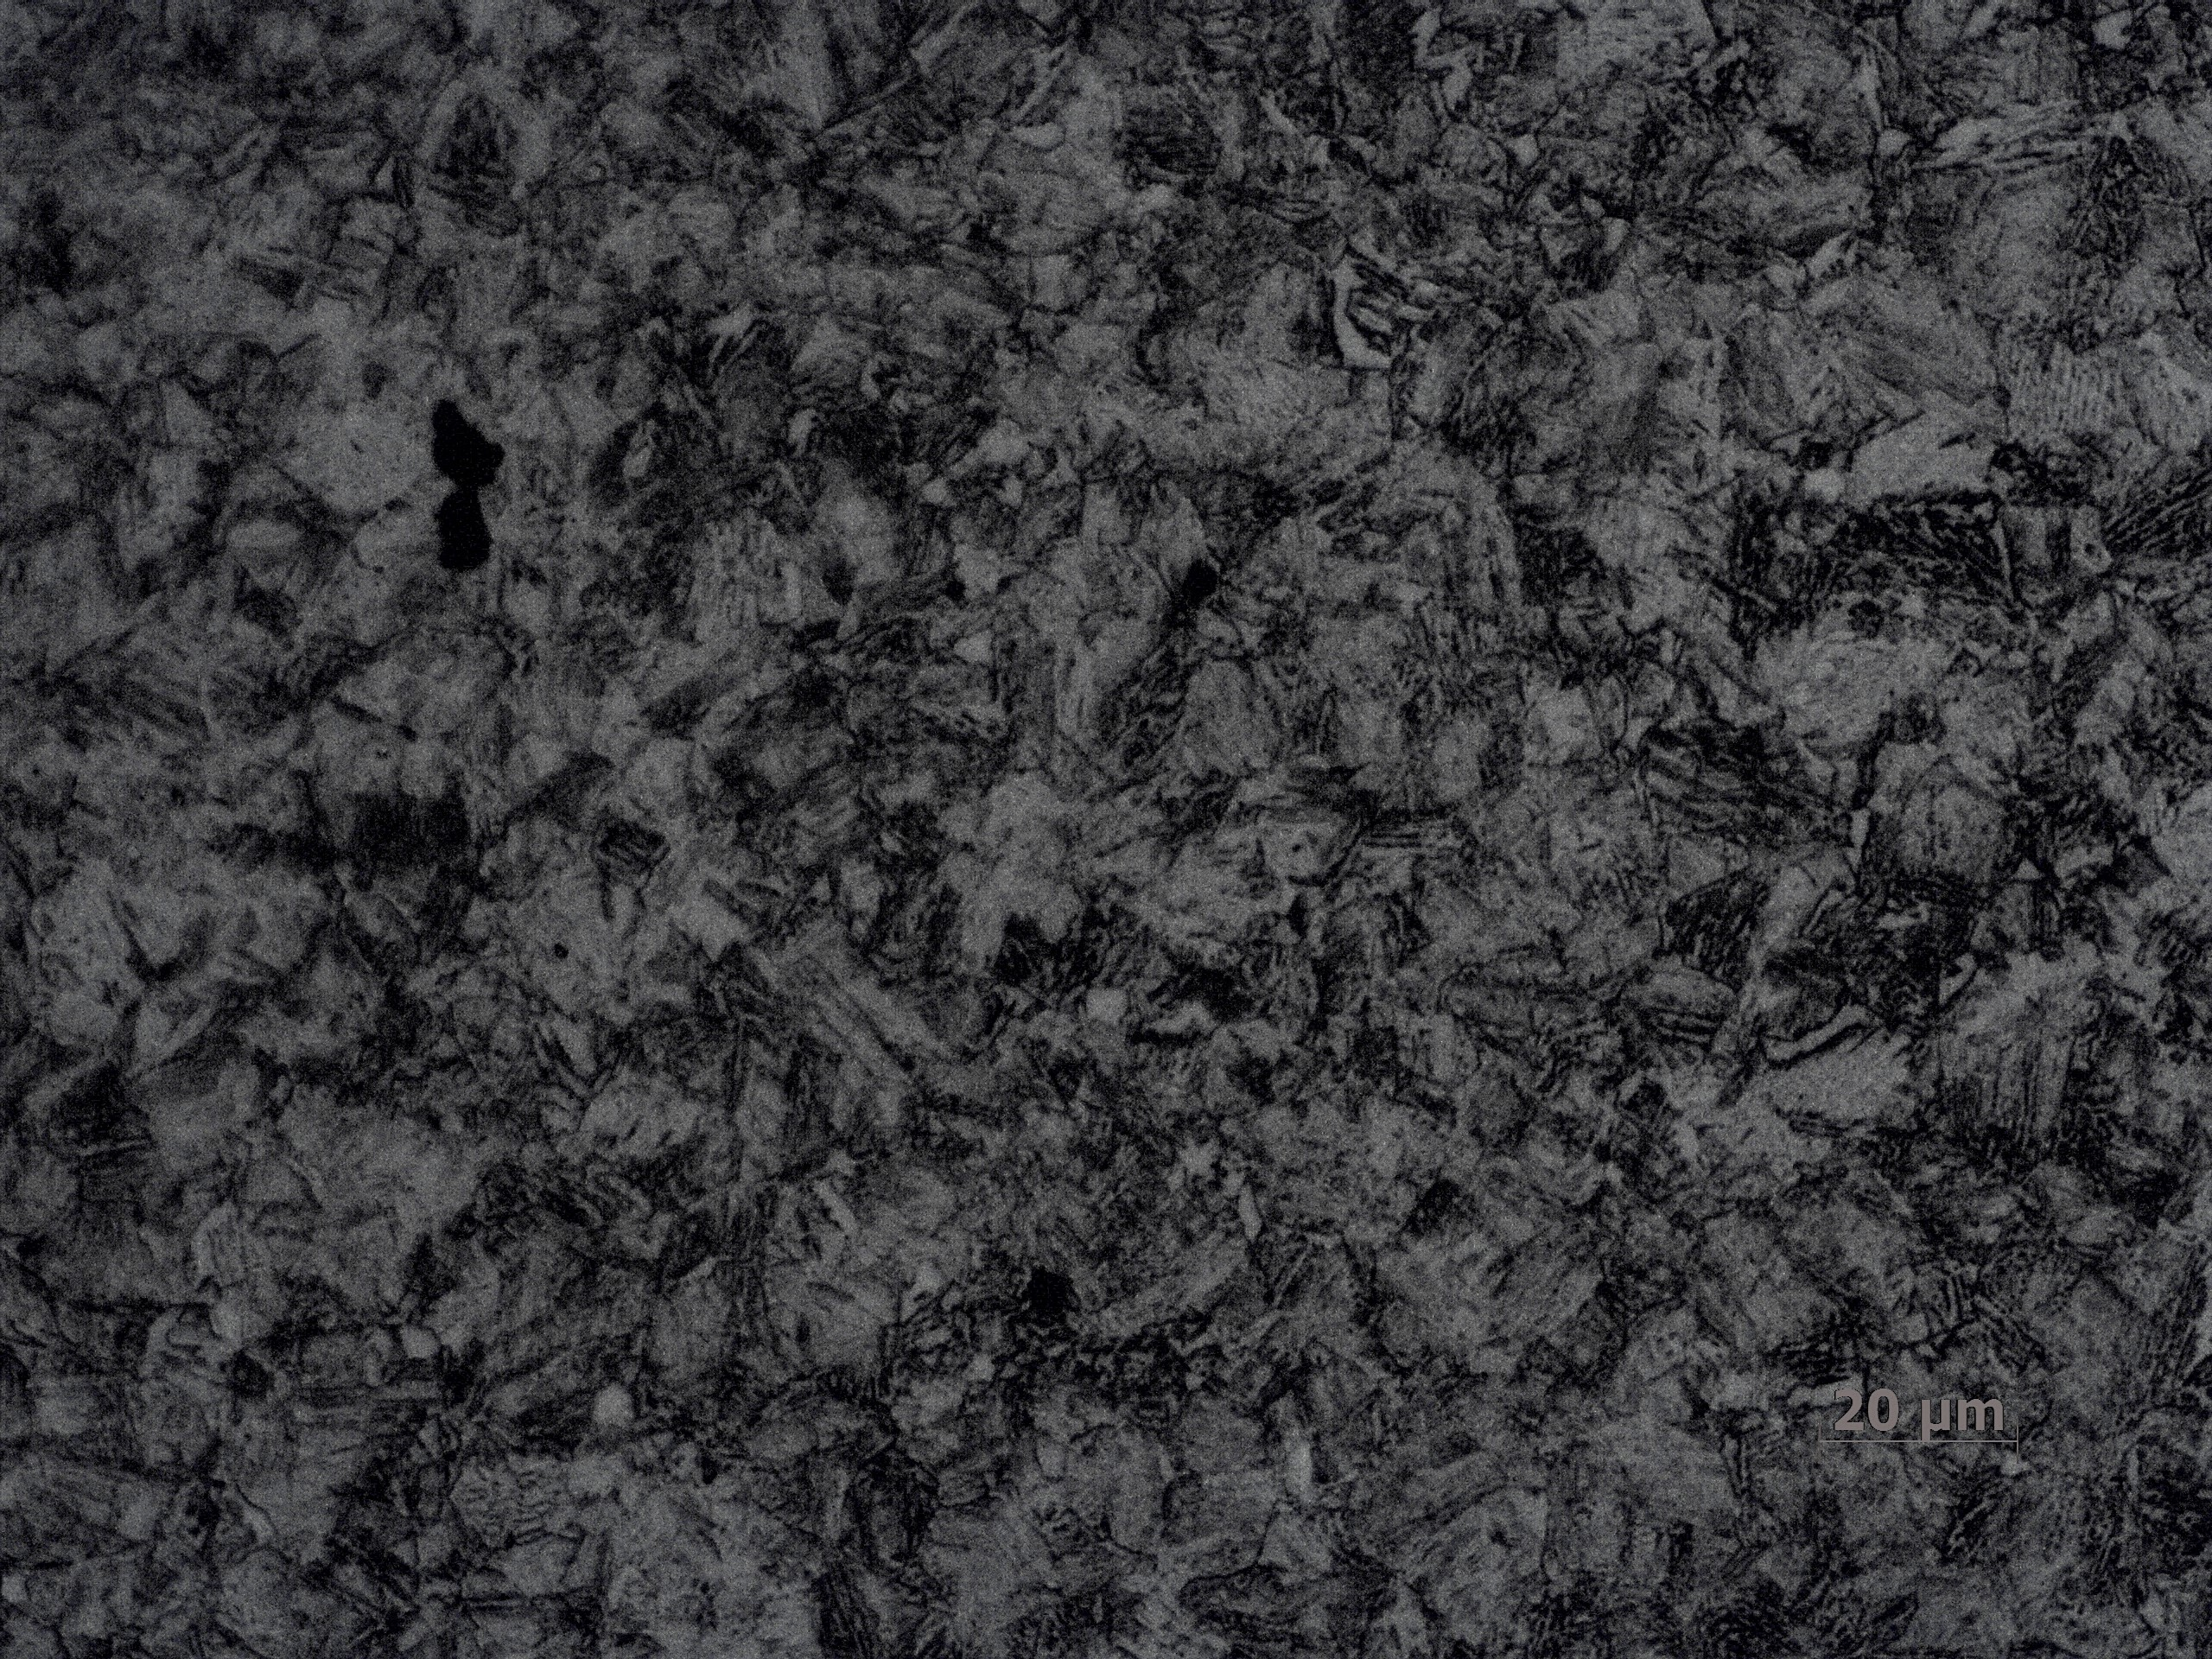
\includegraphics[width=6cm]{20oilguang.jpg}
    \end{minipage}
  }
  \subfigure[扫描电子显微镜1000×]{
    \label{20youdian}
    \begin{minipage}{6cm}
    \centering
    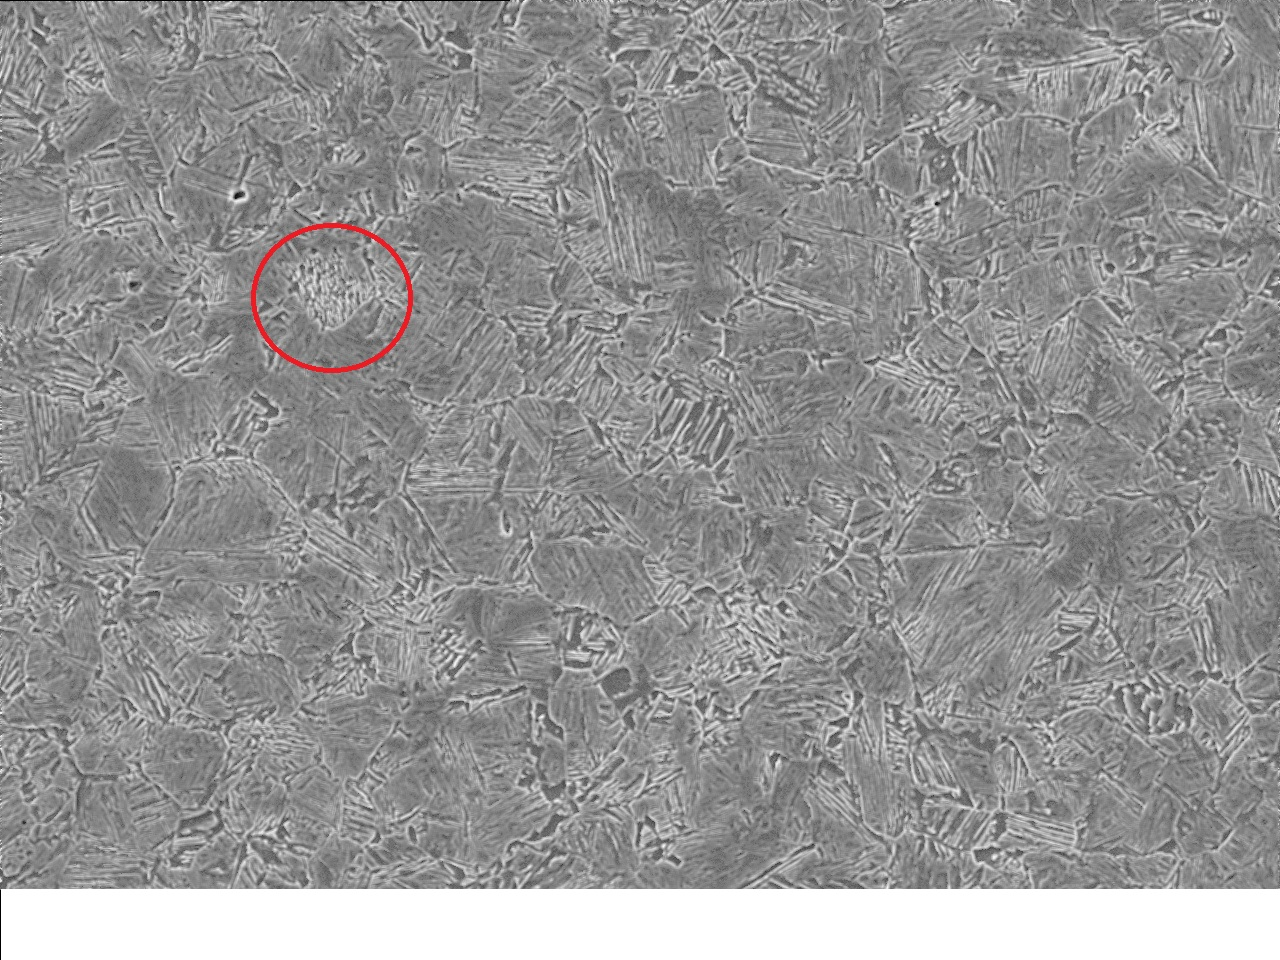
\includegraphics[width=6cm]{20oildian.jpg}
    \end{minipage}
  }
  \caption{20CrMo钢油冷金相照片}
  \label{20water}
\end{figure}
\subparagraph{下贝式体}
在贝氏体相变区较高范围内形成的贝氏体称为上贝氏体
\subparagraph{混合马氏体}
\paragraph{空冷}

\subsubsection{42CrMo钢}
42CrMo钢的CCT曲线如图 \ref{cct42}所示,并根据水冷、油冷及空冷的冷却速度,在图 \ref{cct42}中大致画出冷却曲线:
\begin{figure}[h]
  \centering
  % Requires \usepackage{graphicx}
  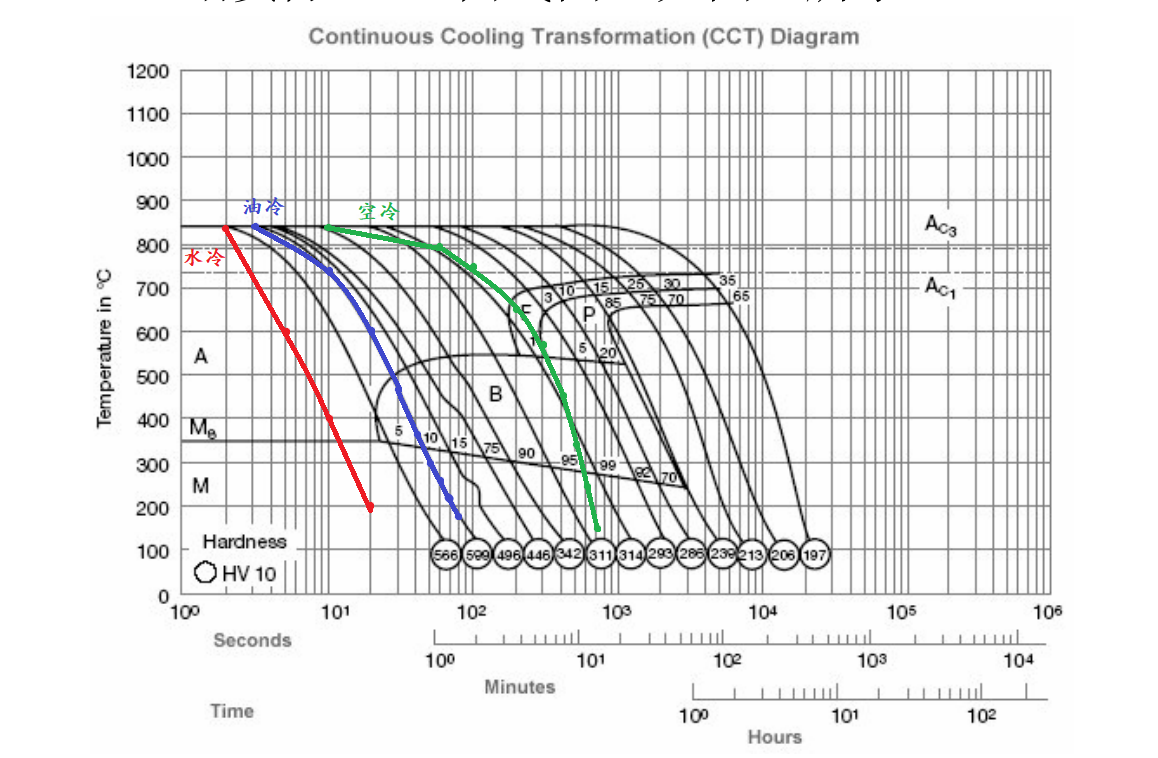
\includegraphics[width=7cm,height=6cm]{cct42.jpg}\\
  \caption{42CrMo钢的CCT曲线}\label{cct42}
\end{figure}

\subsubsection{T10钢}
\begin{figure}[h]
  \centering
  \subfigure[光学显微镜500×]{\label{10guang}
  \begin{minipage}{6cm}
  \centering
  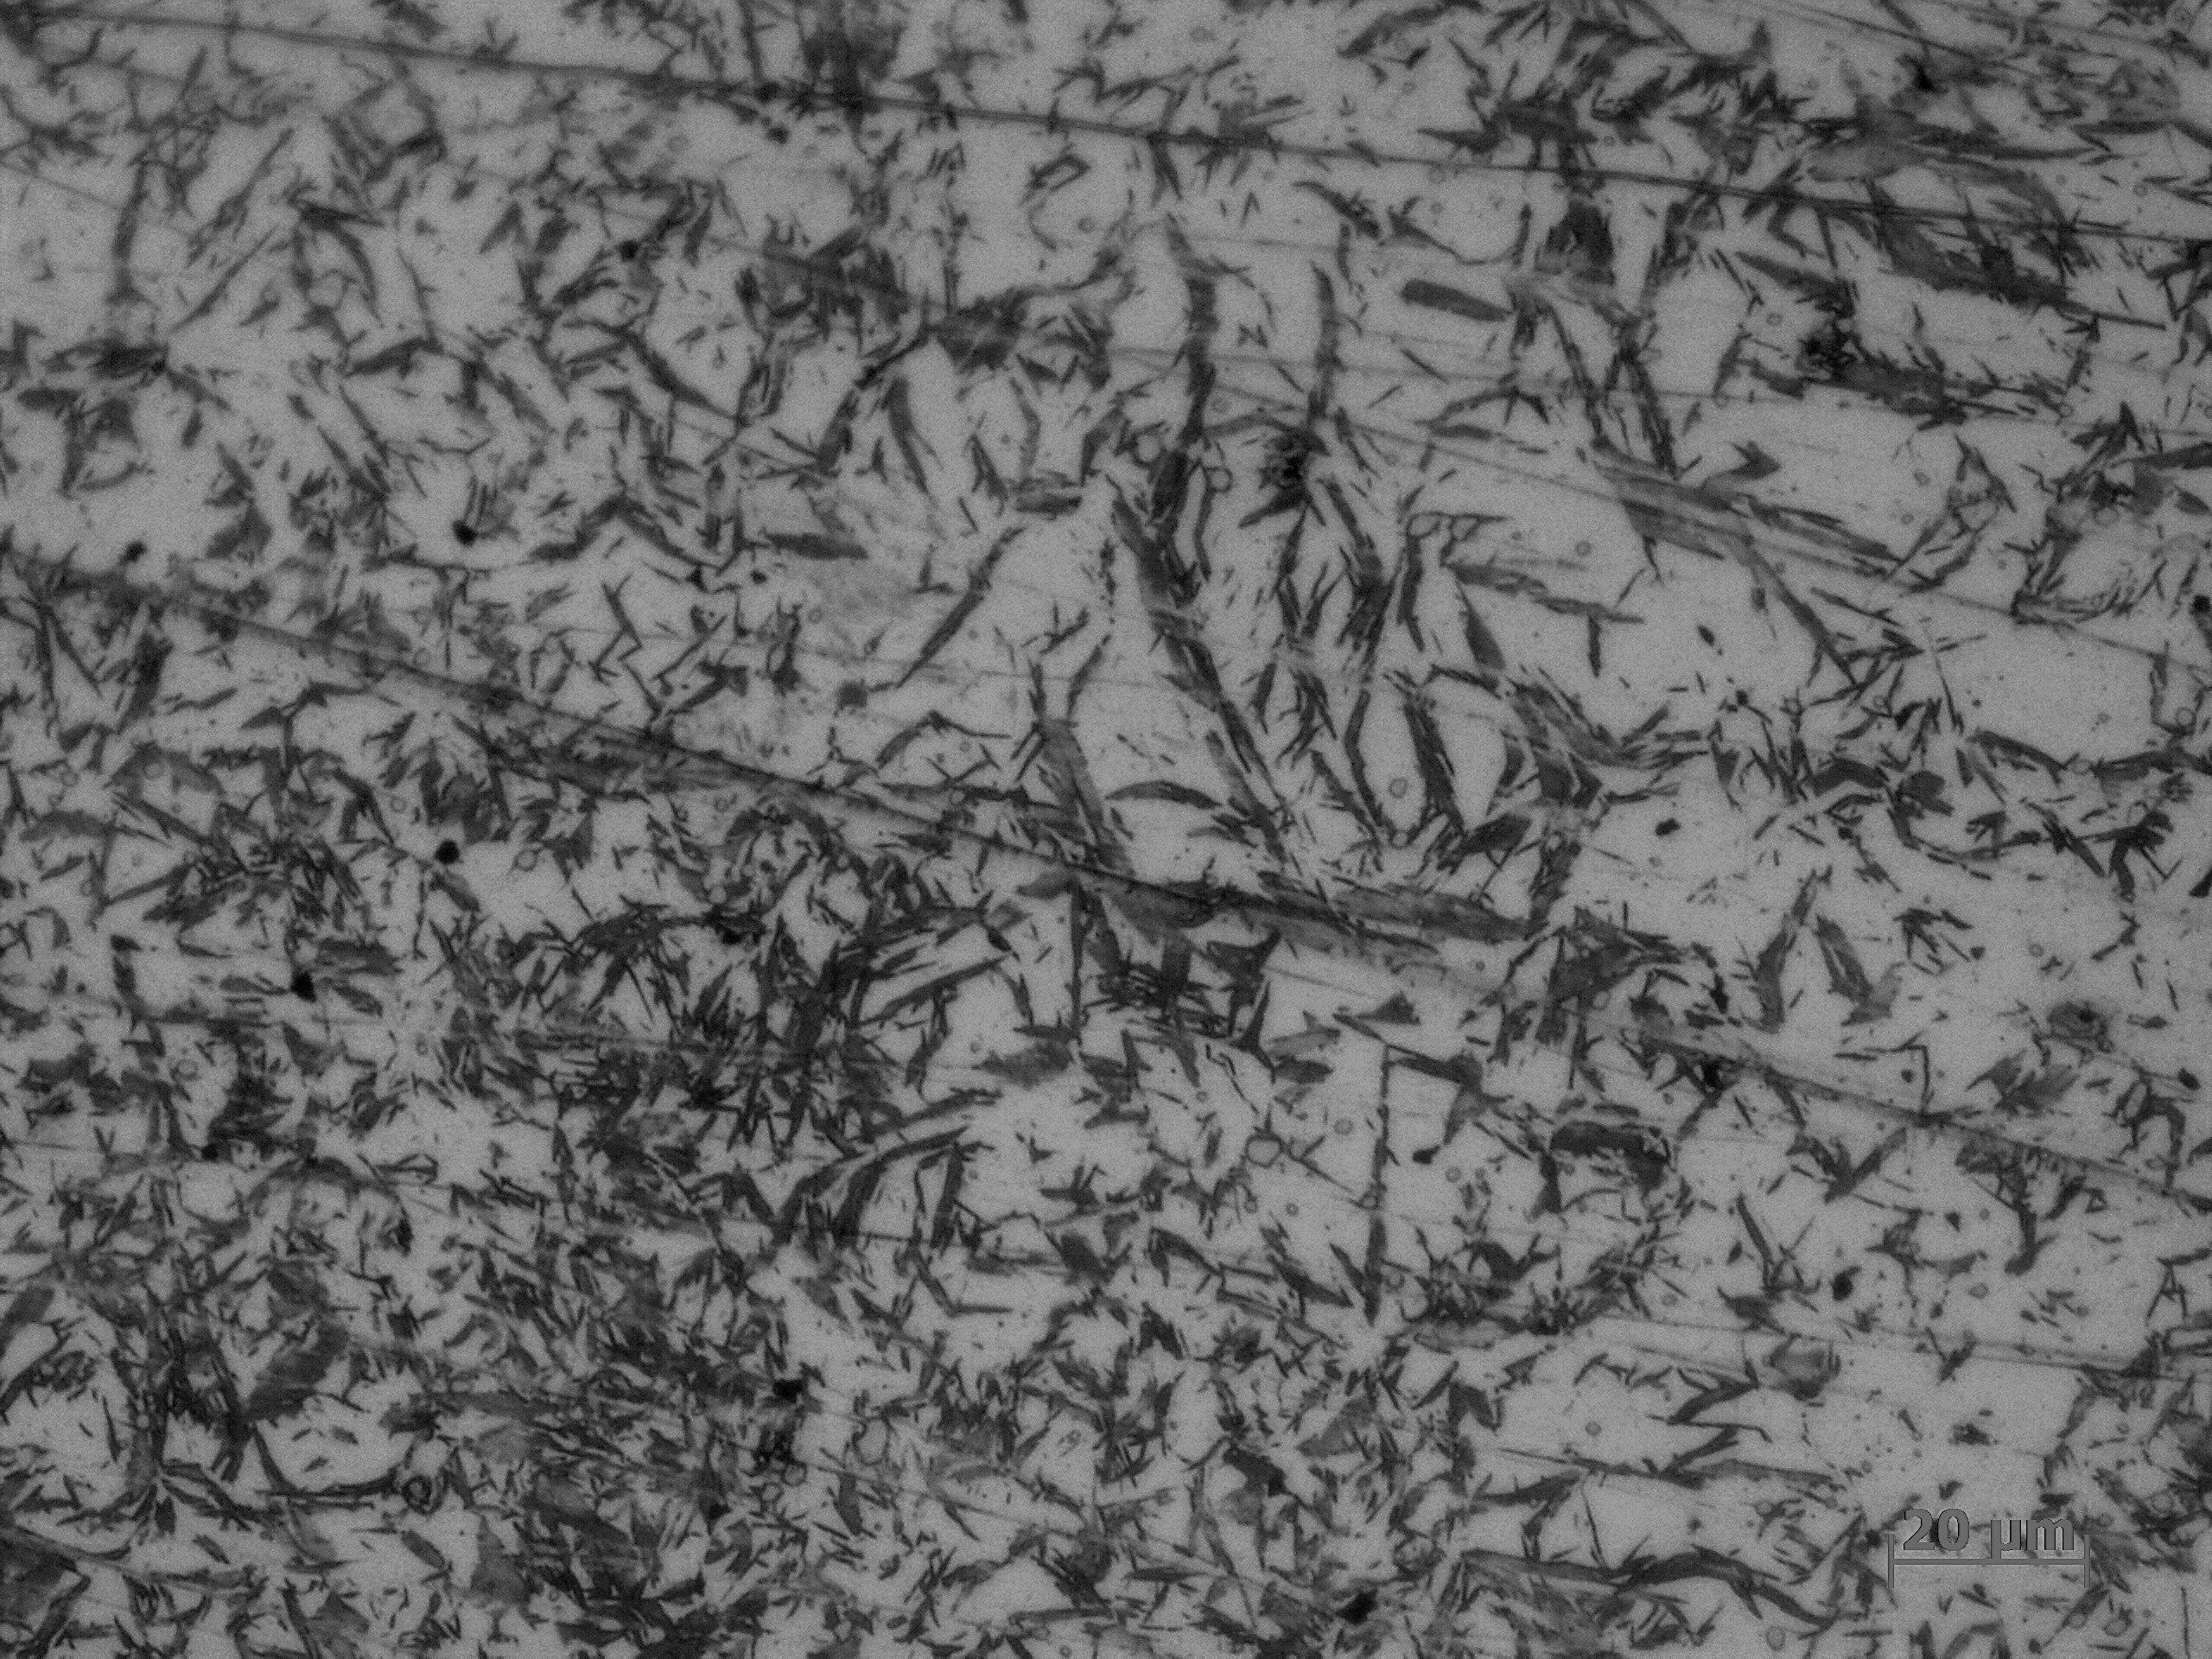
\includegraphics[width=6cm]{10guang.jpg}
  \end{minipage}
  }
  \subfigure[扫描电子显微镜5000×]{\label{10dian}
  \begin{minipage}{6cm}
  \centering
  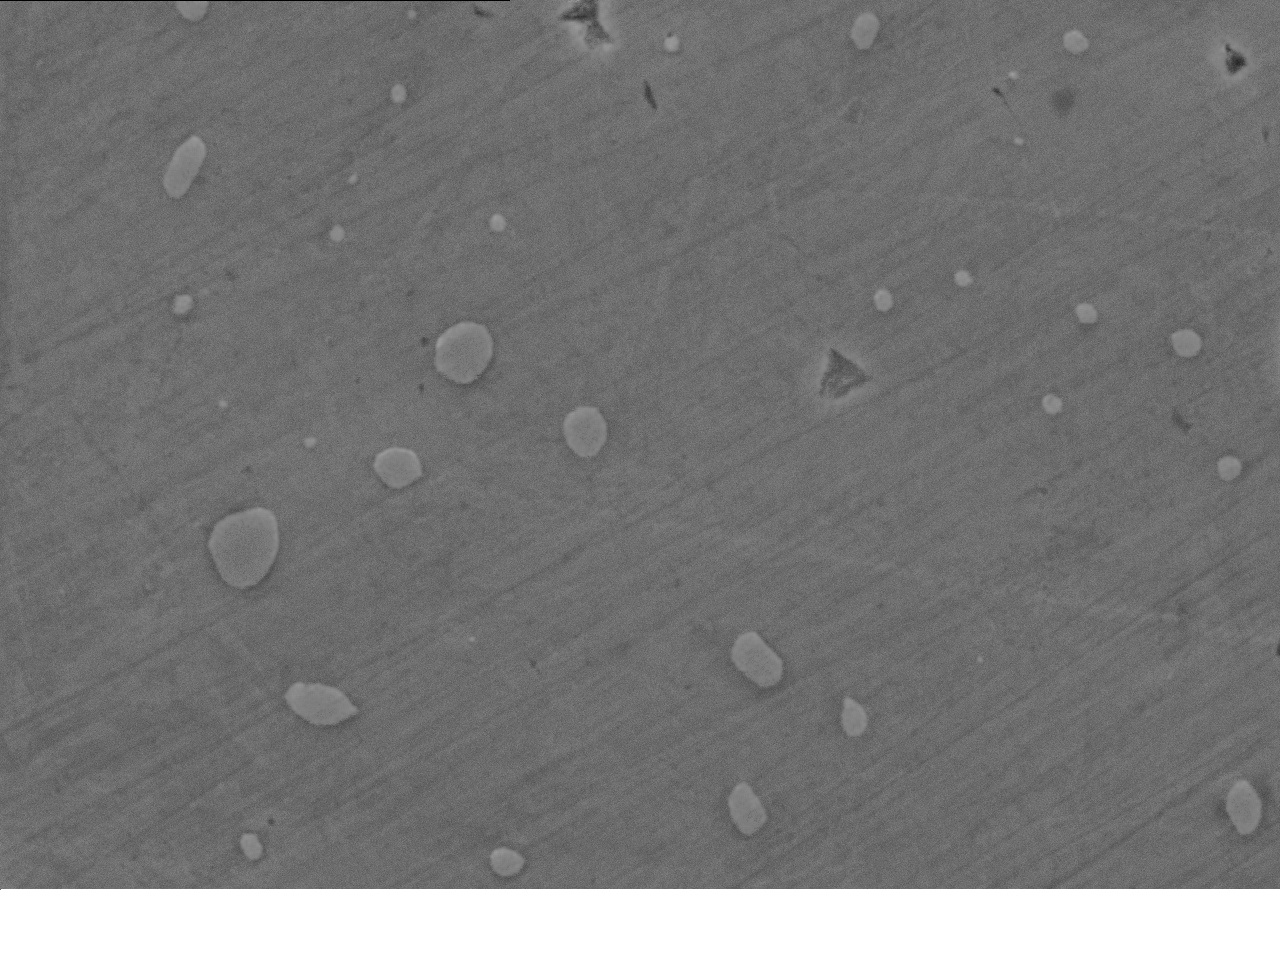
\includegraphics[width=6cm]{10dian.jpg}
  \end{minipage}
  }
  \caption{T10钢油冷金相照片}
  \label{10water}
\end{figure}
\paragraph{水冷}
\subparagraph{裂纹}
在淬火的初期,需要保持较高的冷速超过临界淬火温度,后期需要控制降低内部应力。但实验中水冷速度较快,同时T10钢的含碳量较高,后形成的马氏体片不断撞击先形成的马氏体,由于马氏体形成速度极快,相互撞击,同时还与奥氏体晶界撞击,产生相当大的应力场,在内部将聚集较大的应力,宏观上即可看到一条贯穿样品的裂纹。
\subparagraph{片状马氏体及渗碳体}
片状马氏体是铁基合金中的一种典型的马氏体组织,常见于淬火高、中碳钢中,在图 \ref{10water}的光镜下可以非常清楚的看出针状和竹叶状的马氏体组织。另外其中还存在点状的渗碳体组织,在电镜照片中可以清晰的看出。
\subsection{合金元素的影响}
\subsection{样品硬度分析}
\begin{table}[ht!]
  \centering
  \begin{tabular}{|c|c|c|}
    \hline
    材料 & 冷却方式 & 硬度值(HV) \\
    \hline
    CrMo20 & 水冷 & 401.6 \\
    \hline
    CrMo20 & 油冷 & 346.3 \\
    \hline
    CrMo20 & 空冷 & 191.2 \\ 
    \hline
    CrMo42 & 水冷 & 740.4 \\
    \hline
    CrMo42 & 油冷 & 569.6 \\
    \hline
    CrMo42 & 空冷 & 344.2 \\
    \hline
    T10    & 水淬 & 902.1 \\
    \hline
   \end{tabular}
  \caption{不同冷却条件下的硬度值}
\end{table}

\section{结论}
\end{document}
